\chapter{Exemples de programmes}
\section{Dessiner des maisons}

\begin{figure}[h]
\includegraphics*[width=15 cm]{images/maisons.png}
\caption{Maisons}
\end{figure}
\begin{verbatim}
pour maison :c
repete 4[av 20*:c td 90]
av 20*:c td 30
repete 3[av 20*:c td 120]
fin

pour dep :c
lc tg 30 re :c*20 td 90 av :c*22 tg 90 bc
fin

pour mai
ve lc tg 90 av 200 td 90 bc ct 
maison 3 dep 3 maison 5 dep 5 maison 7 dep 7 maison 10
fin
\end{verbatim} 
\pagebreak
\section{Dessiner un rectangle plein}
\begin{figure}[h]
\includegraphics*{images/rectangle.png}
\caption{Rectangle}
\end{figure} 

\begin{verbatim}
pour rec :lo :la
si :lo=0|:la=0 [stop]
repete 2[av :lo td 90 av :la td 90]
rec :lo-1 :la -1
fin
\end{verbatim} 
\section{Factorielle}
\label{factorielle}
\noindent Rappel: $5!=5\times4\times3\times2\times1=120$ 
\begin{verbatim}
pour fac :n
si :n=0[ret 1][ret :n*fac :n-1]
fin

ec fac 5
120
ec fac 6
720
\end{verbatim} 

\section{Un peu d'écriture...}
\begin{verbatim}
pour ecrire
ct repete 40[av 30 td 9 fcc hasard 7 etiquette [xlogo c'est sympa!]]
fin
\end{verbatim} 

\begin{figure}[h]
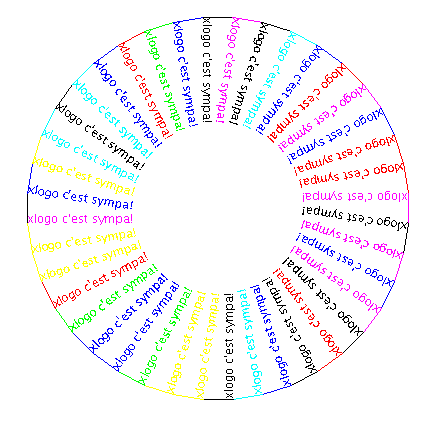
\includegraphics{images/ecrire.png}
\caption{Xlogo c'est sympa!}
\end{figure}
\pagebreak
\section{Et de conjugaison...}
 \subsection{Première version}
\begin{verbatim}
pour futur :mot
ec ph "je mot :mot "ai
ec ph "tu mot :mot "as
ec ph "il mot :mot "a
ec ph "nous mot :mot "ons
ec ph "vous mot :mot "ez
ec ph "elles mot :mot "ont
fin

futur "parler

je parlerai
tu parleras
il parlera
nous parlerons
vous parlerez
elles parleront
\end{verbatim}

\subsection{Deuxième mouture}
\begin{verbatim}
pour fut :mot
donne "pronoms [je tu il nous vous elles]
donne "terminaisons [ai as a ons ez ont]
donne "i 0
repete 6[donne "i :i+1 ec ph item :i :pronoms mot :mot item :i :terminaisons]
fin

fut "parler

je parlerai
tu parleras
il parlera
nous parlerons
vous parlerez
elles parleront
\end{verbatim}
\subsection{Ou alors: Un peu de récursivité !}
\begin{verbatim}
pour fu :verbe
donne "pronoms [je tu il nous vous elles]
donne "terminaisons [ai as a ons ez ont]
conjugue :verbe :pronoms :terminaisons
fin
\end{verbatim}
\pagebreak
\begin{verbatim}
pour conjugue :verbe :pronoms :terminaisons
si vide? :pronoms [stop]
ec ph premier :pronoms mot :verbe premier :terminaisons
conjugue :verbe sp :pronoms sp :terminaisons
fin

fu "parler

je parlerai
tu parleras
il parlera
nous parlerons
vous parlerez
elles parleront
\end{verbatim}
\section{Avec les couleurs}
\subsection{Introduction}
Tout d'abord, quelques explications: vous remarquerez que la commande \texttt{fcc} prend soit en paramètre une liste soit un nombre. Ici, nous allons nous intéresser au codage [r g b] Quésako????\\
Chaque couleur dans XLOGO est codée sur trois composantes, la rouge (red), la verte (green) et la bleue (blue) d'où le nom de ce codage r g b. Les trois nombres donnés dans la liste à la primitive \texttt{fcc} représentent donc dans l'ordre la composante rouge, puis la verte, puis la bleue d'une couleur. Ce codage n'étant pas très intuitif, vous pouvez avoir un aperçu de la couleur obtenue selon le codage à l'aide la boîte de dialogue Options----> Choisir la couleur du crayon.\\
A l'aide de ce codage, il est très facile d'effectuer des transformations sur une image. Par exemple, si l'on veut mettre en niveau de gris une photo couleur, on change la couleur de chaque pixel de l'image en la moyenne des trois composantes [r g b]. Je m'explique: imaginons qu'un point de l'image est pour couleur [0 100 80]. On calcule la moyenne de  ces 3 nombres: $\frac{0+100+80}{3}=60$. On réaffecte alors à ce pixel la couleur [60 60 60]. Cette opération doit être effectuée sur chaque pixel de l'image
\subsection{Passons à la pratique}
Nous allons transformer en niveau de gris une image de 100 pixels sur 100 pixels, il y aura donc $100\times100=10000$ pixels à modifier. Vous pouvez trouver l'image utilisée dans l'exemple suivant à l'adresse: \\
http://xlogo.tuxfamily.org/images/transfo.png\\
Voici comment nous allons procéder: nous allons afficher l'image avec le coin supérieur gauche en [0 0]. Ensuite, la tortue va décrire les 100 premiers pixels de la première ligne puis les 100 premiers de la deuxième etc... A chaque fois, on rapatrie la couleur du pixel avec \texttt{trouvecouleur} puis on modifie la couleur en faisant la moyenne des trois composantes [r g b]. Voici le code correspondant:\\
(N'oubliez pas de changer le chemin dans la procédure transfo)

\pagebreak
\begin{verbatim}
pour li :liste
# renvoie la moyenne des trois nombres [r g b]
donne "r premier :liste
donne "liste sp :liste
donne "g premier :liste
donne "liste sp :liste
donne "b premier :liste
donne "b arrondi (:r+:g+:b)/3
retourne ph liste :b :b :b
fin

pour niveaudegris :c
si :y=-100 [stop]
si :c=100 [donne "c 0 donne "y  :y-1]
# On prend pour couleur de crayon la couleur "moyennée" du pixel suivant
fcc li tc liste :c :y
# On repasse en niveau de gris
point liste :c :y
niveaudegris :c+1
fin

pour transfo
# Vous devez changer le chemin vers l'image transfo.png 
# Ex: frep "c:\\windows chargeimage "transfo.png 

ve ct frep "/home/loic chargeimage "transfo.png donne "y 0 niveaudegris 0
fin

\end{verbatim} 
\begin{figure}[h]
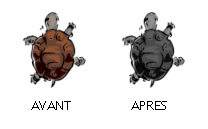
\includegraphics{images/transfo.png}
\caption{XLOGO fait de la retouche d'images....}
\end{figure}

\subsection{Et si on la voyait en négatif??}
Pour changer une image en négaitf, même procédé sauf qu'au lieu de moyenner les nombres r g b, on les remplace par leur complément à 255. Ex: Un pixel a pour couleur [2 100 200], on remplace sa couleur par: [253 155 55]

Seul la procédure \texttt{li} change par rapport à tout de suite:
\pagebreak
\begin{verbatim}
pour niveaudegris :c
si :y=-100 [stop]
si :c=100 [donne "c 0 donne "y  :y-1] 
fcc li tc liste :c :y
point liste :c :y
niveaudegris :c+1
fin

pour transfo
# Vous devez changer le chemin vers l'image transfo.png 
# Ex: frep "c:\\windows\\Bureau chargeimage "transfo.png 
ct ve frep "/home/loic ci "transfo.png donne "y 0 niveaudegris 0
fin

pour li :liste
donne "r premier :liste
donne "liste sp :liste
donne "g premier :liste
donne "liste sp :liste
donne "b premier :liste
retourne ph liste 255-:r 255-:g 255-:b  
fin

\end{verbatim} 
\begin{figure}[h]
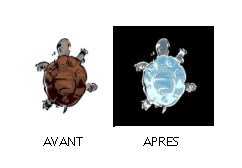
\includegraphics{images/transfo2.png}
\caption{XLOGO se prend pour LE GIMP ...(prétentieux o:))}
\end{figure}

\section{Un bel exemple d'utilisation des listes (Merci Olivier SC)}

Je vous laisse apprécier ce magnifique programme:


\section{Une belle rosace}
\begin{verbatim}
pour rosace
repete 6[ repete 60[av 2 td 1] td 60 repete 120 [av 2 td 1] td 60]
fin

pour belle_rosace
rosace 
repete 30[av 2 td 1]
rosace
repete 15[av 2 td 1]
rosace
repete 30[av 2 td 1]
rosace
fin

fcfg 0 ve fcc 5 ct rosace lc fpos [-300 0] bc fixecap 0 belle_rosace
\end{verbatim} 
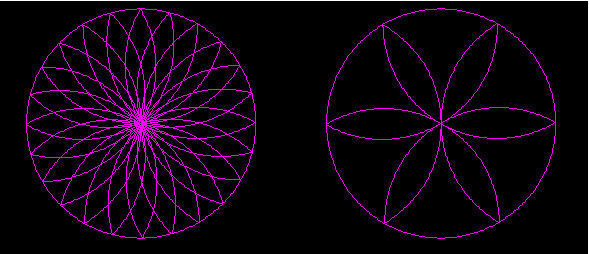
\includegraphics[width=14cm]{images/rosace2.png}

